\documentclass[a4paper,12pt]{article}
\usepackage[utf8]{inputenc}
\usepackage{multirow}
\usepackage{graphicx}
\usepackage{hyperref} 
\usepackage{biblatex}
\usepackage{caption}
\addbibresource{citation.bib}

\hypersetup{
    colorlinks=true,
    linkcolor=blue,
    filecolor=magenta,      
    urlcolor=blue,
}
\title{ Feature Model Test Case Generation using MOEA}
\author{ Team 8 }
\date{December 2019}
\date{\href{https://github.com/youngmi97/FM-SBSE.git}{FM-SBSE.git}}

\begin{document}

\maketitle
\providecommand{\keywords}[1]{\textbf{\textit{Keywords:}} #1}
\begin{abstract}
Increasingly many industries have adopted the concept of Software Product Lines(SPLs), a set of products with common features. Accordingly, the demand for effective ways to test the SPLs has grown as testing all possible products would be impractical in terms of time and cost. Various works have attempted to address this issue by using Genetic Algorithms(GA) to find test sets that are effective with just a small number of representative products. The representative products are selected based on two main testing methods, combinatorial testing and mutation testing. Most existing works, however, incorporate only one of the two methods in finding an ideal test case. In this paper, we propose an extended algorithm that takes into account the cost of testing and the results of both testing methods mentioned above. Results show that incorporating more objectives can give larger set of non-dominating SPLs of the Pareto Front, suggesting better coverage. 


\end{abstract}

\keywords Software Production Line, Feature Model , MOEA 


\section{Introduction}

A feature refers to a specific functionality or attribute of a product that is visible to the user. A collection of products that share common features is called a Software Product Line(SPL). Features of a product are generally represented in a hierarchical tree form known as a Feature Model(FM) and by selecting different features in the FM, a wide variety of products can be created. The adoption of SPL has grown considerably in various industries and the demand for an effective way of testing SPL has increased as well. The main method behind SPL testing is feature testing, which tests whether the products derived from a FM meet certain requirements. Ideally, the most accurate way of testing would be to test all possible products that can be made from the FM. However, considering that many FMs in real life have a large depth, the cost and time of  testing would be infeasible. Hence, only the most representative products are selected to be tested. The criteria used to select these products are based on combinatorial testing for measuring coverage, and mutation testing, which is effective when it comes to fault revelation. 

Most existing work approach feature testing using a single-objective algorithm even though the  problem itself is multi-faceted. Other works that do adopt a multiple-objective approach \cite{MatneiFilho2016} solely concentrate on two objectives, pairwise coverage and number of products. Motivated by such limitations, this paper extends existing algorithms so that they include three objectives, minimal number of products to reduce cost of testing, mutation scores, which indicates the efficacy in detecting faults in the FM and pairwise coverage which insures that most features in the FM are covered by the products in the test set. The approach is implemented using three different genetic algorithms, NSGA-II, SPEA2, and IBEA. The solutions obtained from the respective algorithms are evaluated based on the three objectives to obtain a Pareto Front, a set of non-dominated solutions. In addition, the performance of the algorithms are compared using the hypervolume quality indicator. 

The work is organized as follows. First, the paper explains feature testing and the mechanism behind pairwise testing and mutation testing. Then we review the concept of Multi-objective optimization and Genetic Algorithm(GA) and show how the three genetic algorithms used in the paper differ from each other. Once the background knowledge is given, the paper lays out a detailed description of how the experiment was set up, including which FM was used, how the Feature Model Analyzer(FaMa) was incorporated and how the GA was set up. Following that, the results obtained from the experiment are analyzed leading to conclusions of the work. 



\section{Background}

\subsection{Genetic algorithm}
The concept of Genetic Algorithms (GA) was developed by John Holland on 1960s. GAs are inspired by the principle of Darwinian evolution. The algorithm reflects the process of natural selection where the strong ones are selected for reproduction of offspring of next generation. The fittest individuals have greater opportunity to pass their genes to future generations. 

A solution for the problem is called an individual or a chromosome. Individuals are made of genes which controls distinct features for the solution. The set of individuals is called a population.

GA has 5 phases; Initial population, fitness function, selection, crossover, and mutation.
The algorithm starts with a population, and normally the initial population is created randomly. The fitness function evaluates how fit an individual is. The solutions are ranked by the fitness score. In the selection phase, individuals are selected based on their fitness score. Individuals with higher fitness have more chance to be selected and pass their genes to the next generation. After selecting a pair of parent individuals, a crossover operator is applied iteratively to create offsprings. Genes of fitter individuals are expected to appear more frequently in the population, eventually leading to convergence to a wanted solution. The mutation operator is used to introduce randomness. Normally mutation operator is applied at the gene level. Mutation prevents premature convergence of solution, and maintan diversity within the population. Offsprings after mutation is used to form a new generation. The algorithm terminates if individuals satisfy particular standards or a specific number of evaluations is completed.

GA is a effective meta-heuristic method for solving non-linear problems.

\subsubsection{Initialization}
In our GA, an individual is a single test set comprised of a number of products. The individuals are represented using a bit array of length equal to the number of possible products. Each bit represents a product and its value is 1 if the product is included in the test set and 0 if not. The initial population is created by generating random bit arrays of equal lengths.

\subsubsection {Fitness Function}
Three different fitness functions were incorporated to represent the three objectives of the algorithm. The value of the first function was proportional to the number of products in the individual. Since the goal was to reduce the cost of testing, individuals with a smaller number of products were considered more fit. The other two functions were mutation scores and pairwise coverage which will be further explained in sections 3.2 and 3.3. 


\subsubsection {Selection Operator} 

The Binary Tournament operator was used for selection. 

\subsubsection{Crossover Operator}

Instead of using existing crossover operators, the Product Crossover operator was created for a more effective crossover. The first step of the Product Crossover is to change the representation of the individuals by extracting the indices of ones in the individual, which represent the products included in the test set. Then we performed the crossover on this new representation setting the crossover point as the middle. Finally, the crossed over offsprings are reverted back to the bit array form. The reason why we temporarily change the representation for crossing over is because in bit representation, if the products are concentrated in the first half, then the offspring would be identical to the parent.

\begin{figure}[h!]
\centering
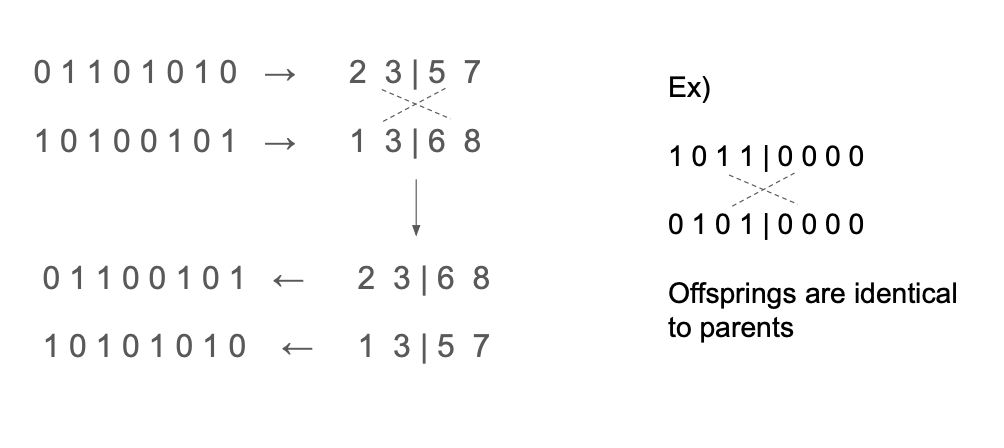
\includegraphics[width=.7\linewidth]{Images/productCrossover.png}
\caption{Product Crossover}
\end{figure}

\subsubsection{Mutation Operator}

The Product Mutation operator is used for mutation. There are three types of mutations in Product Mutation. The add operator adds a new product to the test set. The delete operator removes a product from the test set. The swap operator swaps a product in the test set into another product. The three types of mutations occur with equal probabilities, 1/3 each. After the mutation occurs, we check whether the offspring is a test set with 0 products and if it is, we remove the offspring from the next population and replace it with its parent.  

\subsection{Multi-objective optimization}

Optimization problems involving more than one objective function to be optimized simultaneously are called multi-objective. 

The result of multi-objective optimization is given by set of non-dominated solutions, based on Pareto dominance.There are 3 classes of solutions: $PF_{approx}$ is formed by non-dominated solutions returned by one execution of the algorithm. $PF_{known}$ is the combination of all $PF_{approx}$ obtained through different executions of algorithm, removing dominated and repeated solutions. $PF_{true}$ represents the optimal Pareto Front to the problem. In our case the set is unknown, thus this set was formed by all sets PF known obtained with different algorithms \cite{1197687}. This is in fact an approximation to the real front. 

The generation of the test data sets is a multi-objective problem. In our case, we minimize mutation score, number of test cases, and pairwise coverage simultaneously. 

\subsection{Multi-objective GA}

Variants of GAs are widely used in SBSE to solve multi-objective problems. In our paper, we chose three most representative well known algorithms: NSGA-II, SPEA2, and IBEA. Each algorithms implements different evolution and diversification strategies, hence resulting with characteristic solutions. The algorithms are described below.

\subsubsection{NSGA-II} 

The algorithm NSGA-II (Non-dominated Sorting Genetic Algorithm) \cite{996017} is a multi-objective evolutionary algorithm with strong elitism strategy, and also using crowding distance to maintain diversity. The parameters for the algorithm are the followings: population size, maximum number of evaluations, crossover operator, crossover probability, mutation operator, mutation probability, and selection operator.   
The pseudocode for NSGA-II is described in figure 2. 

\begin{figure}[h!]
\centering
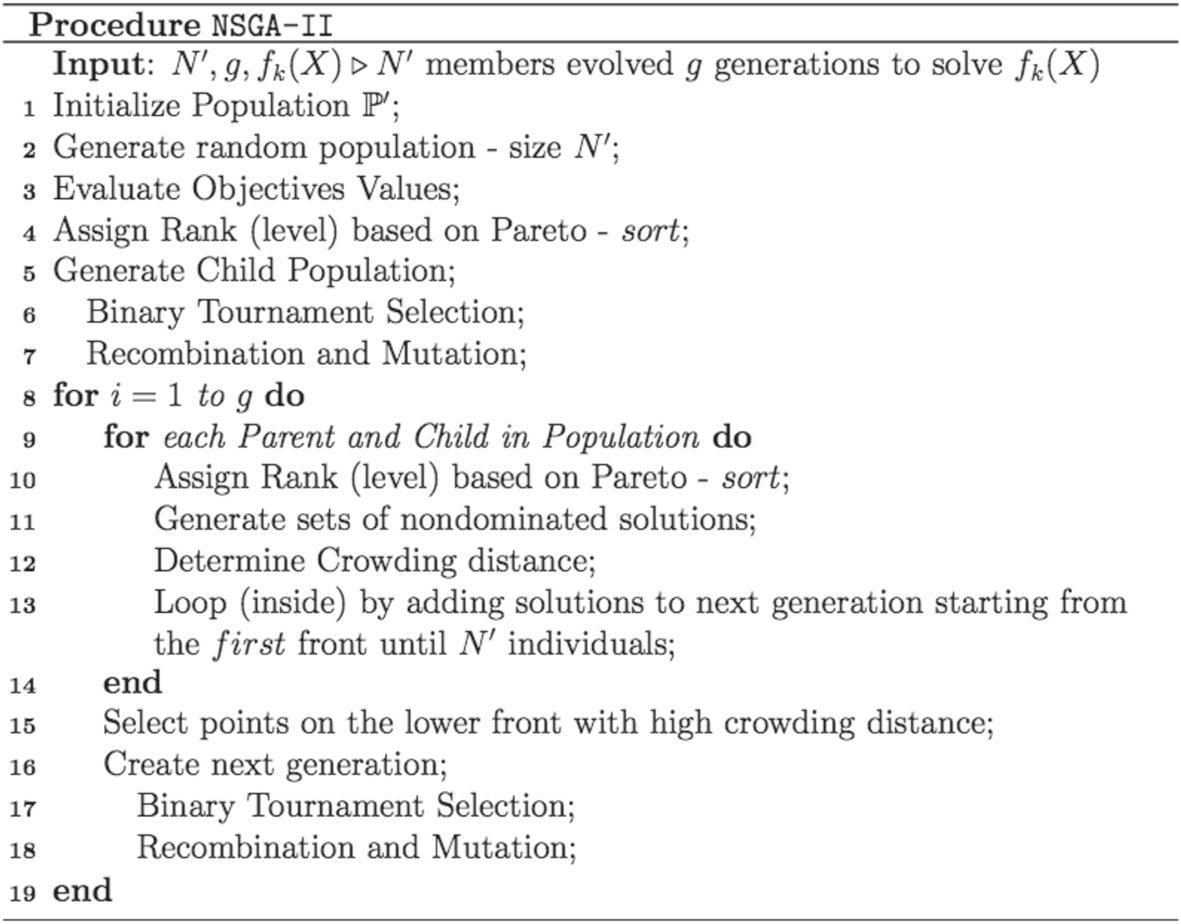
\includegraphics[width=.7\linewidth]{Images/NSGAII.png}
\caption{Pseudocode of NSGA-II}
\label{fig:computerNo}
\end{figure}

\subsubsection{SPEA2} 
SPEA2(Strength Pareto Evolutionary Algorithm) is a multi-objective evolutionary algorithm that keeps archives non-dominated solutions found in each generation. The archived solutions are referenced to calculate the fitness of solutions in the next generation. For this reason, the SPEA2 algorithm requires an additional parameter, archive size. Thus the parameters for the algorithm are the following : population size, maximum number of evaluations, crossover operator, crossover probability, mutation operator, mutation probability, and selection operator.
The pseudocode for SPEA2 is described in figure 3. 

\begin{figure}[h!]
\centering
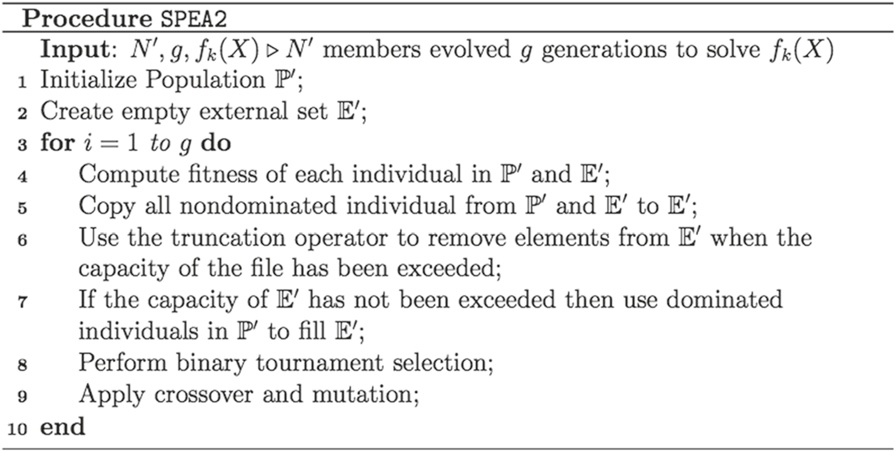
\includegraphics[width=.7\linewidth]{Images/SPEA2.png}
\caption{Pseudocode of SPEA2}
\label{fig:computerNo}
\end{figure}

\subsubsection{IBEA}

IBEA(Indicator-Based Evolutionary Algorithm) is a MOEA based on indicators. Weight is assigned to each solution according to quality indicators. In our case, we used hypervolume as the indicator. The parameters for the algorithm are the following : population size, size of external archive, maximum number of evaluations, crossover operator, crossover probability, mutation operator, mutation probability, and selection operator.
The pseudocode for SPEA2 is described in figure 4. 

\begin{figure}[h!]
\centering
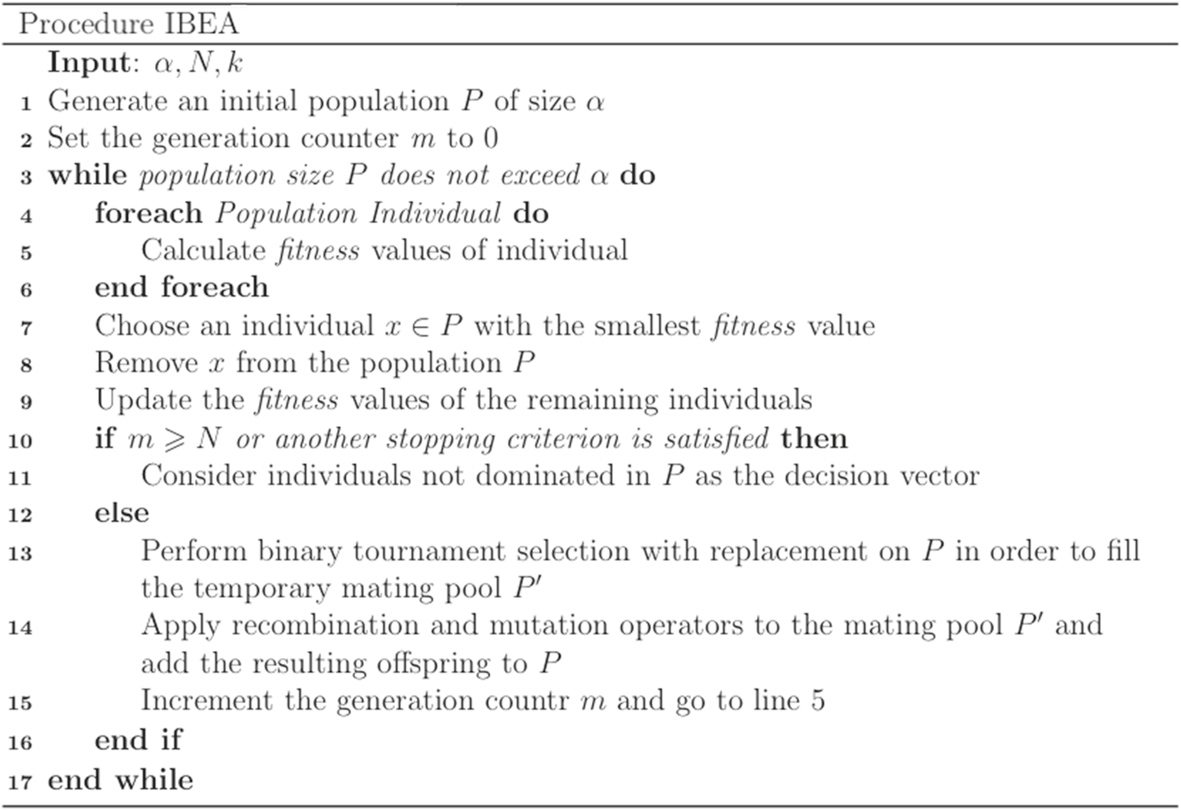
\includegraphics[width=.7\linewidth]{Images/IBEA.png}
\caption{Pseudocode of IBEA}
\label{fig:computerNo}
\end{figure}





\subsubsection{Quality Indicators}

Quality indicators are used to evaluate solutions obtained by each algorithms and compare performance of the algorithms. The indicators are calculated using $PF_{approx}$, $PF_{known}$, and $PF_{true}$. In our work, we evaluated 6 quality indicators: Hypervolume, GD (Generational Distance), IGD (Inverted Generational Distance), Spread, and Epsilon.  
We chose hypervolume as the main quality indicator. Hypervolume measures the coverage area of a known Pareto front on the objective space regarding a reference point. It can measure if a Pareto Front is better than another in terms of dominance relation \cite{1197687}. Hypervolume can be thought to measure both convergence and diversity. The higher the hypervolume, the better the Pareto front is. 

\section{Experiment}
\subsection{Data Processing}
To propose the operators, possible faults in the FM were identified\cite{7102591}. These faults were classified into four categories, described below. The operators in each category are also defined. The FM models were loaded from the open source SPLOT Database \cite{splot}.
\subsubsection{Mutation Operators}
\begin{enumerate}
    \item Incorrect Cardinality of a Solitary Feature: A solitary feature is mistakenly defined:
    \begin{enumerate}
        \item DFL(Decrease solitary feature lower bound, change mandatory feature to optional): $DFL(min, max)$ = $(min - 1, max)$ if $min > 0$
        \item IFL(Increase solitary feature lower bound, change optional feature to mandatory): $IFL(min, max)$ = $(min + 1, max)$ if $min < max$
        \item DFU(Decrease solitary feature upper bound): $DFU(min, max)$ = $(min, max - 1)$ if $min < max$
        \item IFU(Increase solitary feature upper bound): $IFU(min, max)$ = $(min, max + 1)$
    \end{enumerate}
    \item Incorrect Elements of a Grouped Relation: One of the grouped features should not belong to the group, or a solitary feature should be included into a group:
    \begin{enumerate}
        \item AFS(Add feature to a set relation, solitary feature to grouped): $AFS(set(a, b, c), d)$ = $set(a, b, c, d)$
        \item RFS(Remove features from a set relation, grouped to solitary and set relation to binary): $RFS(set(a, b, c, d))$ = $set(a, b, c), d$
    \end{enumerate}
    \item Existence of a Set Relation: Some child features belong to a set relation but they should be defined as solitary features:
    \begin{enumerate}
        \item RSR(Remove a set relation, create solitary and new binary optional relations): $RSR(set(a, b, c))$ = $a, b, c$
    \end{enumerate}
    \item Incorrect Cardinality of a Set Relation: A set relation represents that a certain number of grouped features is included in a product.
    \begin{enumerate}
        \item DRL(Decrease set relation lower bound): $DRL(min, max)$ = $(min - 1, max)$ if $min > 0$
        \item IRL(Increase set relation lower bound): $IRL(min, max)$ = $(min + 1, max)$ if $min < max$
        \item DRU(Decrease set relation upper bound): $DRU(min, max)$ = $(min, max - 1)$
        \item IRU(Increase set relation upper bound): $IRU(min, max)$ = $(min, max + 1)$ if $max < n$, where n is the number of grouped features in a set
    \end{enumerate}
    \item Incorrect Constraint: This class is associated to depends and excludes constraints.
    \begin{enumerate}
        \item CHD(Change a depends constraint): $FDC(dep(a, b)) = dep(b, a)$
        \item FDC(Change a feature of a depends constraint): For each constraint d and a feature f, two mutants are generated: $FDC(dep(a, b), f) = dep(a, f), dep(f, b)$
        \item FEC(change a feature of an excludes constraint): For each constraint and for a feature f, two mutants are generated: $FEC(exc(a, b), f) = exc(a, f), exc(f, b)$
        \item RDC(Remove a depends constraint): $RDC(dep(a, b)) = remove dep(a, b)$
        \item REC(Remove a excludes constraint): $REC(exc(a, b)) = remove exc(a, b)$
        \item CDC(Create a depends constraint): $CDC(a, b, c) = dep(a, b), dep(a, c), dep(b, c)$
        \item CEC(Create an excludes constraint): $CEC(a, b, c) = exc(a, b), exc(a, c), exc(b, c)$
    \end{enumerate}
\end{enumerate} 
\subsubsection{miniFMTS}
We tried to use open source FMTS\cite{article} to test feature models. But its source code was not made available. So we implemented our own mutant generator and mutation tester for feature model, calling it  miniFMTS. In this tool, we couldn't implement few mutation generators that were supposedly present in the original FMTS. There are no CDC, CEC, FDC and FEC operators because implementing them entailed parsing the model XML file much more systematically. So we couldn't store every fault-based mutants during initiation, but we could still generate new constraints that were not present in the input Feature Model.

The mutants are created as individual XML files in the Mutants directory and their equivalence and validity are both tested upon creation. Mutants resulting from the same Mutation Operator are saved in the same Operator directory. These newly created Mutant Feature Models are analyzed with the FaMa Library in the initiation phase.

\subsection{Mutation Testing}
Mutation testing is done by calculating the number of mutants that are "killed" by executing each of the products in the individual suite. A mutant is considered to be dead if the validation procedure of product against the original model differs from that of the mutated model. In other words, when the Mutant generates more products that are different from the original, the more likely it is for that mutant to be killed when executed with the miniFMTS. The fitness score of an individual under Mutation Testing is as follows:

\begin{equation}
Score_{mut} = 1- ( Dead_{mut} / All_{mut})
\end{equation}

\subsection{Pairwise Coverage}
To obtain the pairwise coverage score for each individual, we used the classical coverage method. We first obtained all possible pair of features generated from the original Feature Model and tested how many of these pairs are incorporated in the products of the test suite. The fitness score of an individual under Coverage Testing is as follows:

\begin{equation}
Score_{pair} = Covering_{pair} / All_{pair}
\end{equation}





\subsection{Setup}
The overall procedure of obtaining the true Pareto front of Software Product Lines (set of products) was achieved through initiating the environment for the GA to take place. In the initiation, the mini FMTS was utilized to load the Feature Model to be examined, and it also helped to generate mutants and consequent list of products associated with the original and the mutated models. Also, tuple of all possible feature pairs were generated in the initiation phase. These data were modularized to formulate fitness functions for both pairwise coverage of the SPL and its Mutation Score. 

Running the MOEA with two objectives – Mutation Score and Set Size minimization – can be done from \emph{two-obj-test.java} from the \emph{jmetal.core} package of \emph{JMETALHOME} directory, and running the MOEA with three objectives – with pairwise-coverage score minimization – can be done from \emph{three-obj-test.java} of the same directory.

Each of the runs will generate the resultant Pareto Fronts of each of the MOEA algorithm, together with the Known Pareto Front generated by combining the 3 MOEAs. Text files with the prefix 'FUN' saves the coordinates that make up each of these fronts.



\section{Results}
Our solutions for two-objective are shown as in Figure 5, Figure 6, and Figure 7 each of which are Pareto fronts we obtained on three different feature models. The Pareto fronts are ranked from the population which is combined with all three algorithms NSGAII, SPEA2, and IBEA. 

\begin{figure}[h!]
\centering
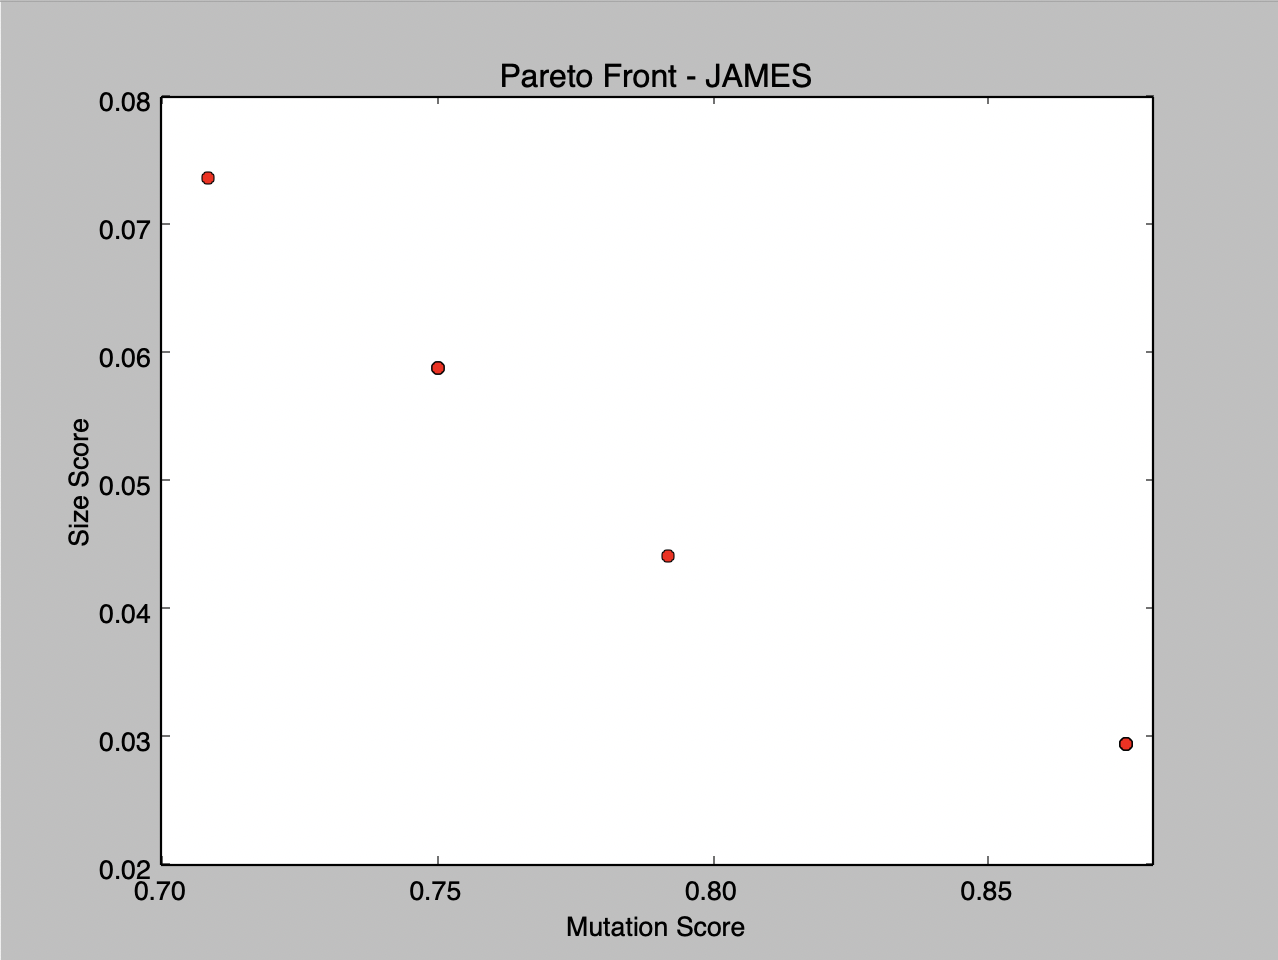
\includegraphics[width=.7\linewidth]{Images/JAMES.png}
\caption{Two-obj solution for JAMES}
\label{fig:computerNo}
\end{figure}
\begin{figure}[h!]
\centering
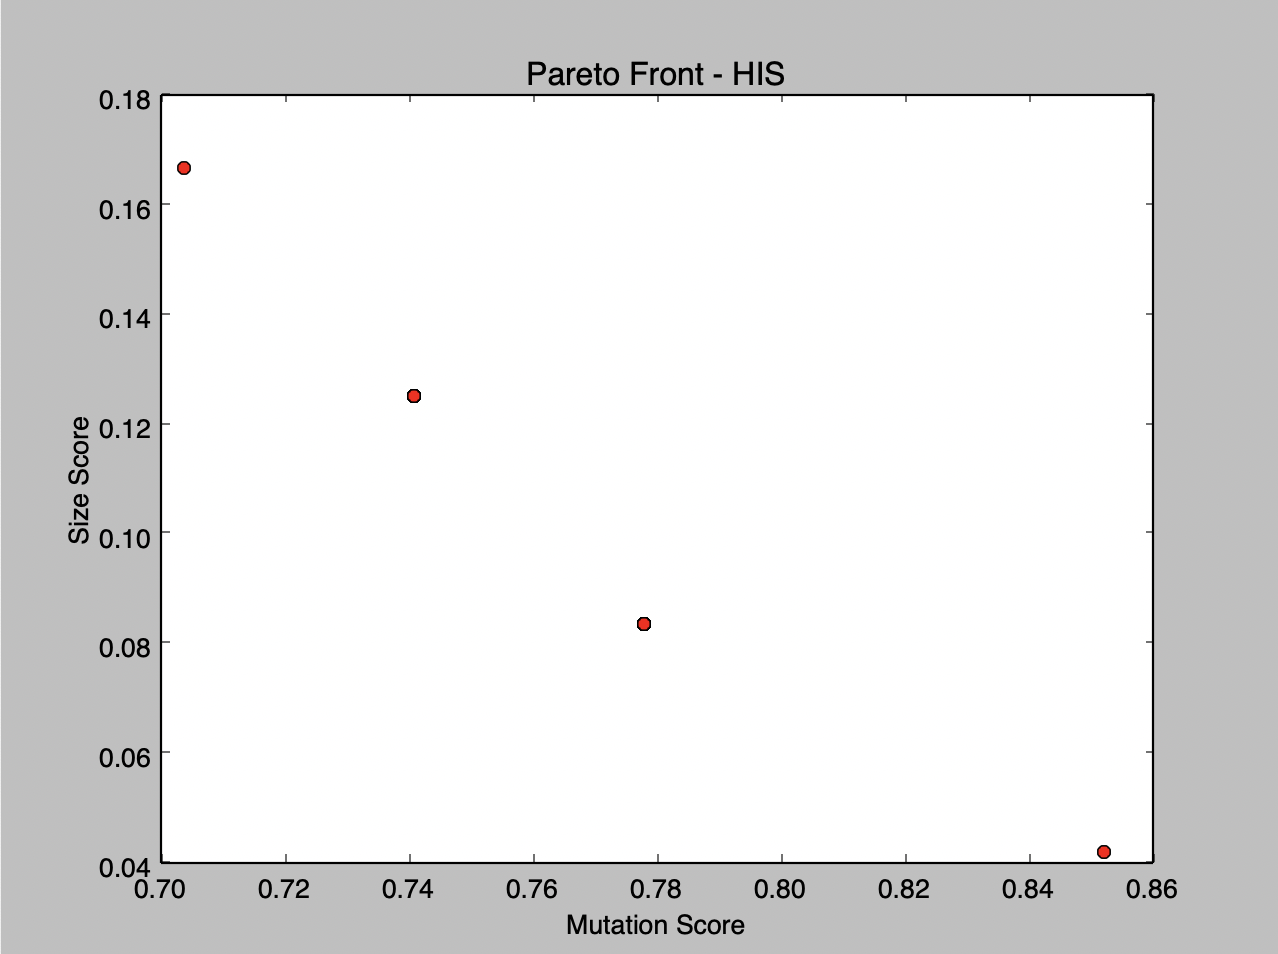
\includegraphics[width=.7\linewidth]{Images/HIS.png}
\caption{Two-obj solution for HIS}
\label{fig:computerNo}
\end{figure}
\begin{figure}[h!]
\centering
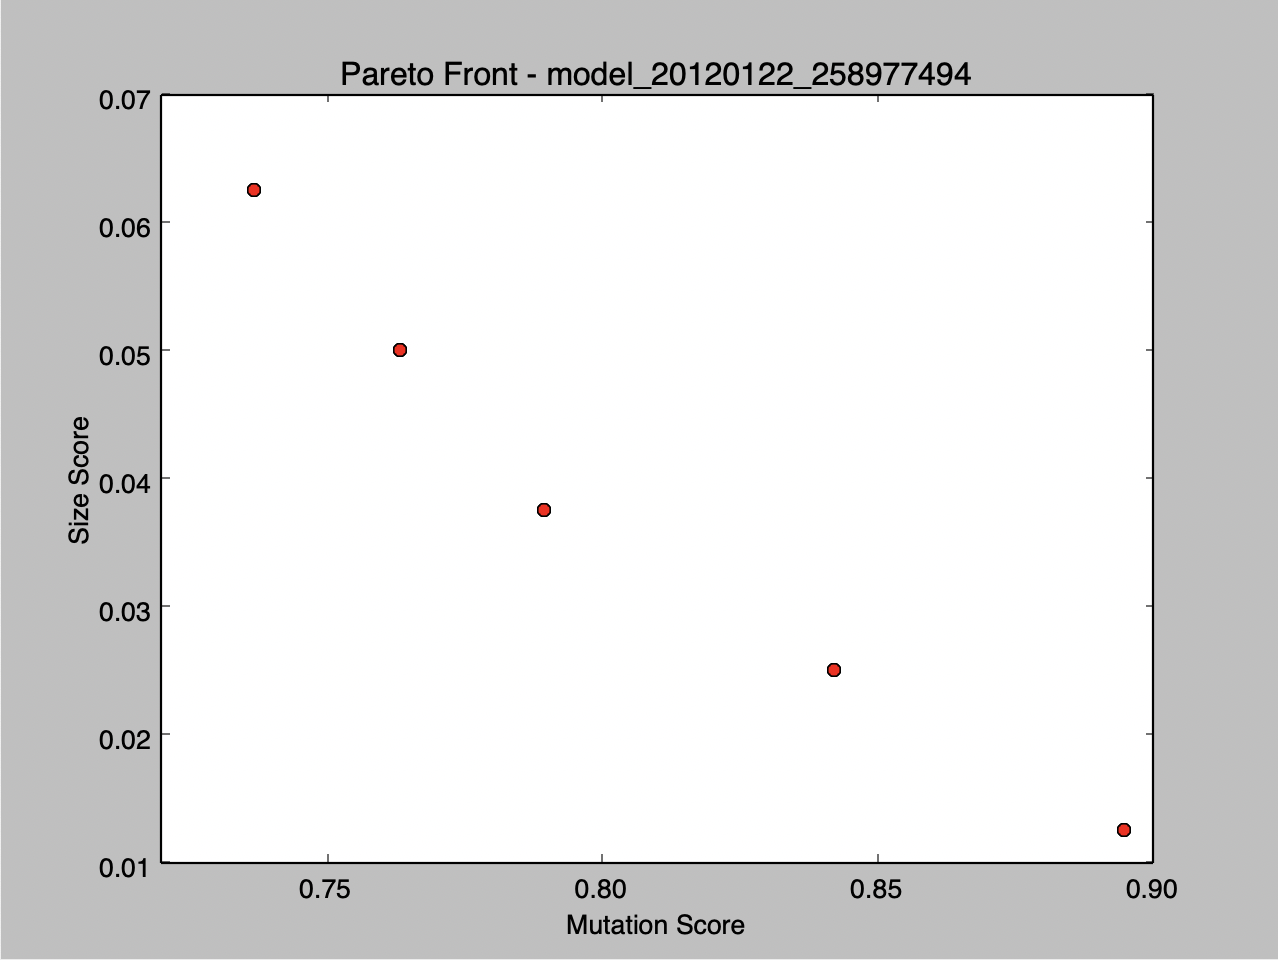
\includegraphics[width=.7\linewidth]{Images/model.png}
\caption{Two-obj solution for custom model}
\label{fig:computerNo}
\end{figure}

Table 1. shows the number of Pareto front knowns that were obtained. The first column denotes the models have been tested. The second column is the amount of real fronts($PF_{true}$) and the third column is the fronts that we obtained from the algorithms($PF_{known}$). From the three models that we tested, for two of the feature models, $PF_{known}$ are in at least half of the $PF_{true}$. However, for two-objective the evalutation converges to only 4-5 Pareto fronts. When the feature models were mutated using various mutation techniques, the mutation occurred for one technique at a time and there is a possibility that the mutated model was too similar to the original model itself. \par

\begin{table}[h!]
\centering
\begin{tabular}{|l|l|l|}
\hline
\textbf{Feature Models}    & \textbf{PF True} & \textbf{PF Known} \\ \hline
JAMES                      & 8                & 4                 \\ \hline
HIS                        & 15               & 4                 \\ \hline
model\_20120122\_258977494 & 10               & 5                 \\ \hline
\end{tabular}
\caption{Pareto Fronts - two-objective}
\label{table:computerNo}
\end{table} \par


Our three-objective solution was as follows. Figure 8 shows a simple 3D graph of the Pareto fronts. Compared to two-objective, three-objective solution had better coverage of Pareto fronts. In Table 2, $PF_{known}$ covers 11 of the 13 $PF_{True}$. This ensures there are various fitness values as the Pareto fronts so there are more selections to make for the test cases. If test size is more important then the fronts that are closest should be selected and if the efficency is more important then the fronts closer to the right y axis should be selected.\par
\begin{table}[h!]
\centering
\begin{tabular}{|l|l|l|}
\hline
\textbf{Feature Models} & \textbf{PF True} & \textbf{PF Known} \\ \hline
JAMES                   & 13               & 11                \\ \hline
\end{tabular}
\caption{Pareto Fronts - three-objective}
\label{table:computerNo}
\end{table}
\begin{figure}[h!]
\centering
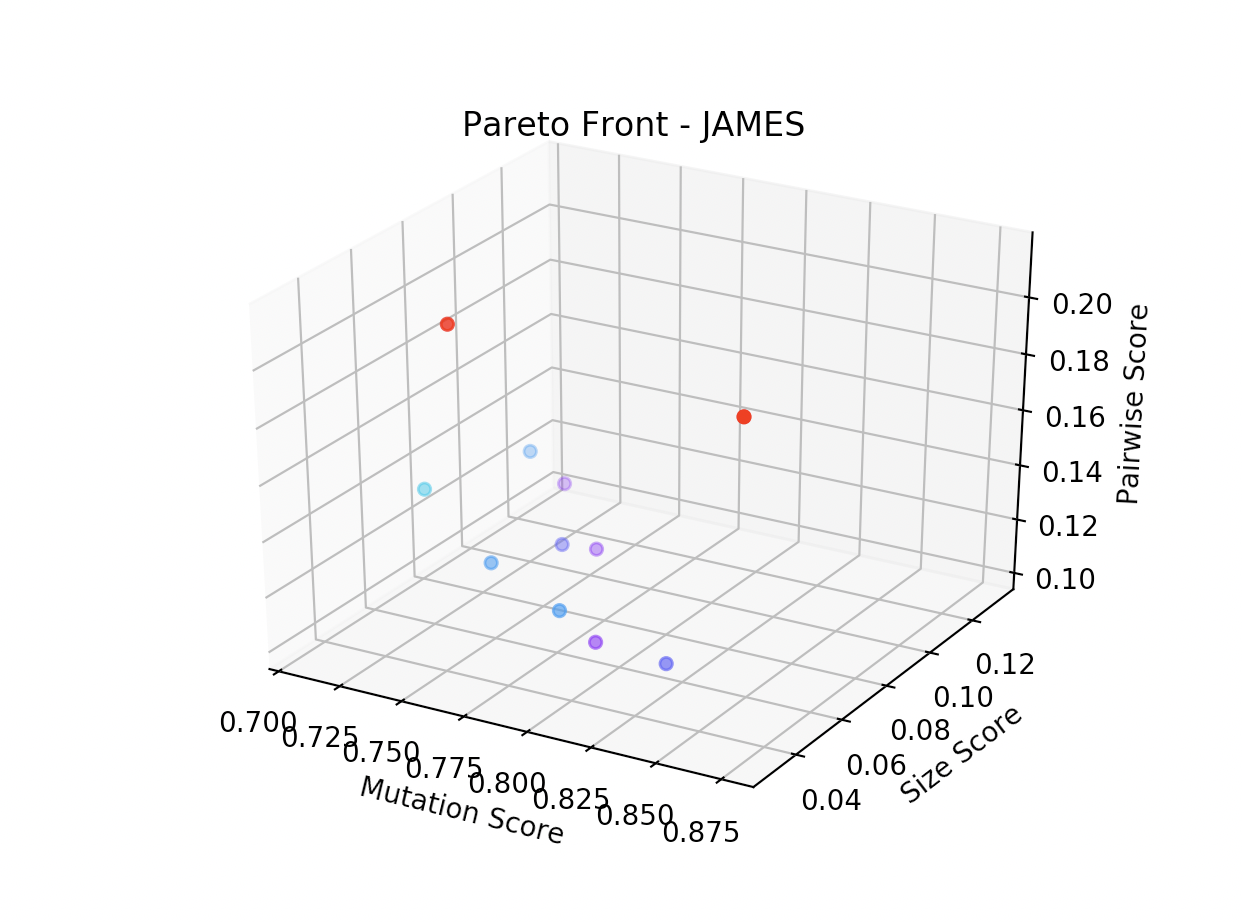
\includegraphics[width=.7\linewidth]{Images/3D.png}
\caption{Three-obj solution for JAMES}
\label{fig:computerNo}
\end{figure} \par

\begin{table}[h!]
\centering
\begin{tabular}{|l|c|c|c|}
\hline
\multirow{2}{*}{\textbf{Feature Models}} & \multicolumn{3}{c|}{\textbf{Hypervolume}} \\ \cline{2-4} 
                                         & NSGAII        & SPEA2        & IBEA       \\ \hline
JAMES                                    & 0.08          & 0.5          & 0.41       \\ \hline
HIS                                      & 0.41          & 0.16         & 0.41       \\ \hline
model\_20120122\_258977494               & 0.16          & 0            & 0.46       \\ \hline
\end{tabular}
\caption{Hypervolumes - two-objective}
\label{table:computerNo}
\end{table}
\par

\begin{table}[h!]
\centering
\begin{tabular}{|c|c|c|c|}
\hline
\multirow{2}{*}{\textbf{Feature Models}} & \multicolumn{3}{c|}{\textbf{Hypervolume}} \\ \cline{2-4} 
                                         & NSGAII        & SPEA2        & IBEA       \\ \hline
JAMES                                    & 0.5           & 0.67         & 0.34       \\ \hline
\end{tabular}
\caption{Hypervolumes - three-objective}
\label{table:computerNo}
\end{table}

One of the most important values that needs to be focused in the hypervolume. The best hypervolume means statistical significance. In Table 2, the hypervolume values are shown for each algorithm when it was tested on the three models with two-objective experiment. It is evident that IBEA has the highest hypervolume among all three algorithms. This denotes that IBEA contributed most to obtaining the combined Pareto fronts. And alternatively, clearly SPEA2 algorithm was more important in finding the Pareto fronts for three-objective. Perhaps if the Pareto fronts were tested and combined in fashion of emphasizing the algorthim that are more significant for two and three-objective, then we might expect better results.


\newpage
\printbibliography


\end{document}
